%%%%%%%%%%%%%%%%%%%%%%%%%%%%%%%%%%%%%%%%%%%%%%%%%%%%%
\chapter{Introduction}
\label{chapter:intro}

The interaction between conductors and musicians
is a sophisticated form of non-verbal communication.
While the expressions used in conducting have no strict rules,
most gestures performed by experienced conductors are understood by
adequately experienced musicians.
Modelling this complex conductor-musician interaction
requires understanding the fundamental principles behind the communication.
Once the relevant features are identified,
it is possible to implement a system that
follows the movements of a conductor
by capturing and interpreting relevant data.
By combining this conductor following with
a musical score and a sound synthesis system,
an interactive sonic experience can be created.

\section{Conducting Gestures}

While some forms of musical conducting have been around for hundreds of years
\cite{modernconductor},
the developments that lead to the modern form of conducting
were driven by the increasing size and complexity of symphonic scores
in the late nineteenth century \cite{gallops2005}.
The task of the modern conductor is to mold an interpretation
by guiding the musicians to play a musical score according to his or her vision.
This is done not only by non-verbal gestures
using body postures, hand movements, eye contact and facial expressions,
but also using verbal instructions during rehearsals.

Studying conducting from a scientific, data based approach,
is a rather recent development.
Sousa \cite{sousa1988} was among the first,
performing a study in 1988,
which investigated the use of musical conducting emblems,
and their interpretation by instrumental performers.
Sousa used videotaped conducting gestures,
which he presented to university, high school and junior high school students,
to study which gestures could be classified as conducting emblems,
non-verbal acts with precise meaning and
a common interpretation among instrumental performers.
He concluded that 38 out of the 55 studied gestures
were recognised by over 70\% of the subjects,
with the recognition rate having a strong correlation
with the experience level of the musicians.

While some conducting gestures can be easily analysed,
and do have a commonly recognized meaning,
to really understand how the communication between
conductors and musicians works,
one has to study the whole life cycle of a conducted performance --
preparations made by the conductor before rehearsing with the musicians,
rehearsal with musicians,
and finally the actual performance.
Konttinen \cite{konttinen2008} studied
conducting as a practical and sociological activity
in her dissertation \textit{Conducting Gestures}.
She came to the conclusion that the main purpose of all
conducting gestures become apparent in a social situation --
a rehearsal, performance or conducting class --
where the communicational situation includes both the gesture
and the social context in which it is used.
Therefore the meaning of conducting gestures are
heavily influenced by their social context --
the musicians affecting the way the conductor performs,
and the conductor affecting the way the musicians interpret the gestures.
Especially the rehearsal situation,
where the conductor needs to make the meaning of his gestures obvious,
is crucial for founding the basis for successful gestural communication.

\section{Gesture-Based Human-Computer Interaction}

When using gestures for human-computer interaction (HCI),
the device used for gathering data plays a big role
in the capabilities and limitations of the system.
Early gesture systems were based on input from
a camera or a specially made input device,
such as a light-pen and screen combination \cite{turk2002}.
Recent developments in technology --
such as the popularization of touchscreen smartphones --
have made gestures as a form of HCI
a part of everyday life for an increasing amount of people.
Judging by the over 600 IEEE conference publications related to gestures in 2011,
it is obvious that gesture based systems are an active field of research.

Depth sensor equipped motion sensing input devices --
such as the Mictosoft Kinect \cite{kinect_overview} --
represent a recent trend of incorporating gesture based interaction
into consumer electronics.
Interaction with applications using these devices
does not require touching or wearing any equipment,
and thus applications have the potential to provide
a very natural gestural user interface.
However, the complexity of the subject lies in extracting
meaningful information out of the raw motion data provided by these devices.
For surveys on related literature,
see \cite{Moeslund2006} and \cite{Weinland2011}.

User interfaces that do not require an artificial input device
and are based on models that occur as natural to users,
are sometimes referred to as natural user interfaces (NUI),
and the act of using such an interface Natural Interaction (NI).
Most NUIs are built on top of an application
that presents the user with rather abstract data,
with no established set of gestures for operating on it available.
A conductor follower, however,
is quite the opposite of the usual case,
as it is based on an already defined --
albeit somewhat varying -- set of gestures.

\section{Tempo Following}

One of the most fundamental musical parameters communicated
to the orchestra by the conductor, is tempo.
Tempo is not, however, a simple parameter to follow
in a musically pleasing way.
To understand the concepts related to tempo following,
one has to look at two separate problems:
conductor-performer synchronization,
and expressive timing.
Furthermore, since tempo is essentially the
first derivative of position,
and both are communicated via the same means --
by conducting beats --
synchronizing both tempo and position is not trivial.

Beat synchronization has been studied in
both laboratory \cite{LuckSloboda2008, LuckSloboda2009}
and musical rehearsal situations \cite{luck2006}.
These studies provide insight into
beat induction, i.e.
what features are used to
derive beats from continuous motion.
The studies conducted in rehearsal situations
have shown that realistic conducting
situations differ from laboratory beat induction tests.
However, these studies have been rather limited,
and do not provide any insight on
how absolute tempo or tempo changes
affect the synchronization.

Expressive timing refers to the mostly subtle
differences in timing that occur over phrases.
These changes are used by the musician as a means of expression.
While the average tempo may be steady across a piece of music,
the length of a transcribed note duration (e.g. quarter note)
will differ depending on its position in the score.
This minute variance in timing has been studied,
and many studies have concluded,
that simple parabolic \textit{tempo curves} are not sufficient
for representing expressive timing
\cite{Desain1993, Kirke2012}.
It has also been discovered,
that expressive timing is
dependent on the absolute tempo \cite{Desain1993, Desain1994},
and is thus in no way trivial to model.

Several systems for producing expressive timing --
based on rule sets, machine learning, or statistical models --
have been developed.
A comprehensive overview of such systems can be found in \cite{Kirke2012}.
These systems aim at adding tempo and loudness variation
to raw notation data,
in order to make it sound more human-like.
Given that the tempo in the performance does not differ much
from the notated tempo,
these features can be added to a score file beforehand.


\section{Expressive Sound Synthesis}

Music is fundamentally a form of human expression,
and thus expressiveness a fundamental property of music.
Therefore one could argue that the ultimate goal of sound synthesis should be to support
the expressive motives of the composer and performer of the music.
However, most control parameters available in sound synthesis systems
are not related to the expressive properties of the produced sound,
but are rather based on the time-frequency properties of the signal.
Various studies have been made on the relation between
descriptive and emotional concepts,
and the time-frequency properties of sound.
The studies have covered both musical cues,
such as tempo, loudness and articulation \cite{juslin2000cue},
and the timbre of individual notes \cite{moravec2005}.
While these studies do present clear results,
the largest problem in applying them in a conductor follower system
is deriving the emotional descriptors from the
gestures of the conductor. 

The majority of motion based expressive sound synthesis implementations
have been novel approaches which do not model any existing form of musical expression.
Some have concentrated on using emotional data
extracted from the motion of the user,
to control music in a way that the
emotional features of the music would match those of the user \cite{friberg2004},
while others have provided means to create mappings
between arbitrary motion data and sound features \cite{kia2004}.
Because bringing out expressive features of music is a crucial part of conducting,
a conductor follower is a rather natural candidate for
an expressive sound synthesis system.

\section{Thesis Overview}

This thesis is based on the development of
a conductor follower system,
which uses motion capture and sound synthesis techniques
to provide an interactive experience of conducting a virtual orchestra.
In this chapter the central concepts behind
the work in this thesis are discussed.
Chapter \ref{chapter:conductor_following} discusses
previous similar systems, and gives an overview on the current system.
Chapter \ref{chapter:motion_capture} describes the
methods related to motion capture used for
gesture and expressive feature detection.
Chapter \ref{chapter:score_following}
formalizes the principles
and defines the methods used for following the musical score.
Chapter \ref{chapter:sound_synthesis}
discusses sound synthesis related design and
implementation choices.
Chapter \ref{chapter:implementation_details}
highlights the most relevant details
in the implementation of the system.
Chapter \ref{chapter:discussion}
evaluates the results of the project,
discusses recommended further work on the subject,
and provides a conclusion of the thesis.

%%%%%%%%%%%%%%%%%%%%%%%%%%%%%%%%%%%%%%%%%%%%%%%%%%%%%
\chapter{Conductor Following}
\label{chapter:conductor_following}

Over the years, several conductor follower systems for
performance, educational and research use have been designed and implemented.
These systems follow conductor gestures
and produce or modify music based on the input.
This chapter provides a brief overview of previous systems,
and introduces the system to be implemented together with its design rationale.

\section{Previous Work}

Conductor following systems implemented in the past
can be roughly classified based on four features:
the types of sensors used for capturing gestures,
the methods used for analysing the gesture data,
the level of control they provide, and
the type of sound synthesis they use.

This section provides a brief overview on how these four features
have been implemented in previous systems.
As more comprehensive overviews can be found elsewhere --
one of the latest and most detailed being \cite{Fabiani2012} --
the overview here will be kept brief.

\subsection{Sensors for Gesture Capture}

While the history of conductor following systems
can be traced back to
early computer performance control systems
where score parameters could be modified during playback
by using control interfaces which do not resemble a conductor's baton \cite{Buxton1980},
the first system that tracked a baton-like wand
was developed in 1983 \cite{Haflich1983}.
The system was able to analyze conducting gestures performed with the wand,
and control the tempo and dynamics of a score.
Since then, several similar systems have been developed,
utilizing a multitude of tracking methods,
including the following:
\begin{itemize}
\item systems that measure the capacitance between a baton and an "antenna",
\item accelerometer based systems,
\item magnetic sensors,
\item infra red based systems,
\item video analysis from a regular video stream, and
\item direct measurement of the conductor's body movements with
sensors attached to the conductor.
\end{itemize}
In addition to tracking the movements of the baton or hands,
breath and gaze sensors have also been used.
For examples of projects using each sensor type,
the reader is asked to reference \cite{Fabiani2012}.

Capturing the relevant data from the conductor's gestures
provides the raw input to the system.
While the quality and quantity of this data
sets the baseline for what can be done
in the later stages of processing,
the method used for acquiring the data
is very loosely coupled to the rest of the system.

\subsection{Methods for gesture analysis}

The methods used for analysing the raw data
provided by the sensors define the
mode of interaction between the conductor and the system.
The most fundamental differentiation between different systems
can be made based on their mode of output:
whether the method produces
a set of continuously varying parameters,
or a stream of discrete events based on detecting discrete gestures.
Most systems combine both types of analysis methods.
While it is possible to use
heuristics to extract data \cite{Ilmonen1999, Morita1991},
also hidden Markov models (HMMs) \cite{Usa1998, Kolesnik2004, Lee2006} and
artificial neural networks (ANNs) \cite{Ilmonen1999, Bruegge2007}
have been used.
All these methods can be used to produce both discrete events
and continuous values for parameters.

Since both hands have distinct roles in conducting,
the methods used for gesture analysis also differ between the hands.
Since the right hand is used for conducting the tempo
and is in continuous motion,
both continuous parameters --
such as articulation and dynamics related features --
and discrete events --
such as beats, fermatas and beat pattern changes --
can be extracted from its motion.
The left hand, however,
is usually used only for discrete gestures.

The features described above are all rather low level.
However, it is possible to also extract
higher level features from the conductor's movement.
While the output of the analysis differs from
the lower level feature extraction,
the methods used for analysis will be somewhat similar,
using methods such as heuristics, HMMs or ANNs.
The difference between these modes of control
will be discussed in more depth in the next section.

\subsection{Performance Control}

Fabiani et al. define three levels of performance control in \cite{Fabiani2012}:
direct control, model-based performance control,
and high-level control via semantic descriptors.
The distinction between these modes is necessarily fuzzy;
many systems use a combination of the three levels.
In direct control systems,
the user is in direct control of the performance parameters,
such as tempo, dynamics, articulation, and instrument section balance.
Model-based performance control combines the input from the conductor
with a performance model.
Performance models include
e.g. changes in dynamics and tempo
for achieving expressive phrasing.
In model-based systems
there is always a trade-off between stability and sensitivity --
i.e. if much weight is put on the model,
the system will not be very sensitive to the input,
while too much weight on the input
can cause very large deviations from the model.
Most of the previously implemented conductor following systems
use a combination of direct and model based control.

The highest level of control utilizes semantic descriptors --
such as emotional expressions --
to control the performance.
This requires mapping the descriptors to both motion features
and performance features,
which allows first translating motion features to
descriptors and then applying relevant performance features
based on the descriptors extracted.
While studies have produced clear results for
the relation between semantic descriptors
and musical and tonal qualities \cite{moravec2005, juslin2000cue},
the mapping of conducting gestures to semantic descriptors
has not been studied as extensively.

\subsection{Synthesis}

Once the performance parameters have been generated
based on the gestures of the user,
they need to be applied to the score.
The methods implemented in previous systems can be classified
into two categories:
synthesizing the output from a score file using a synthesizer,
or applying modifications to a pre-recorded performance.
While the former can obviously be implemented very flexibly
using any synthesis method available,
the number of options for implementing the latter is more restricted.
The methods used for modifying pre-recorded performances
include time-frequency manipulation
and mixing different recordings \cite{Borchers2004}.

\section{Design Rationale}

If the real life interaction between a conductor and musicians
were to be modelled as closely as possible,
it would require providing a feedback channel
equivalent to the verbal communication from conductor to musicians.
This channel could then be used to teach the
style of the specific conductor to the system.
In other words, when the system misinterprets some gesture,
the conductor could correct this interpretation by 
providing the correct interpretation via the feedback channel.
This would make it possible for the system to
learn the style of the conductor over time,
using machine learning techniques.
Implementing such a system would, however,
be too large an effort for the scope of this project.
Instead, a more static and general heuristics based system is
considered and implemented.

The main goals of the project can be
summarized with the following statements:
\begin{enumerate}
\item The system should be usable without wearing or holding external equipment.
\label{item:usable_without_equipment}
\item The system should be usable by anyone familiar with conducting, without having to provide extensive instructions on usage.
\item The system should react to conducting like a real orchestra.
\label{item:sould_react_like_real_orchestra}
\item The system should produce sound that resembles a real orchestra.
\end{enumerate}
Out of these goals,
only the \spellRefOrdinal{item:usable_without_equipment}
is easily evaluated,
while the rest are more complex,
at least point \ref{item:sould_react_like_real_orchestra}
requiring expert evaluation.

\section{System overview}

The system can be broken down to four functional components:
motion tracking, score following, sound synthesis
and visualization.
Since the synthesis is not implemented in this project,
we need to communicate with the synthesis component
via a third party application programming interface (API).
For this reason, a plugin component is required.
Since the plugin standard used in the project
(discussed in more detail in section \ref{sec:vst})
provides a method of creating user interfaces (UIs),
the visualization will be part of the plugin.
This leaves us with three modules
to be implemented:
the \textit{Motion Tracker}, \textit{Score Follower} and \textit{Plugin}.
A a data flow oriented overview of the architecture
can be found in figure \ref{fig:architecture}.

\begin{figure}
\begin{center}
\includestandalone{images/architecture}
\caption{
Data flow oriented architecture overview.
Sharp-cornered rectangles depict software modules and
ellipses depict data sources.
The round-cornered rectangle is reserved for the user.
A dotted outline implies that the item was not
implemented or specified in this project.
}
\label{fig:architecture}
\end{center}
\end{figure}

The \textit{Motion Tracker}
takes depth sensor input,
analyzes the body movements of the conductor,
and produces a stream of events and
a set of continuously varying motion parameters.
These events and parameters describe
those features of the conductor's movement,
which are relevant to conductor following.

The output of the Motion Tracker is then analyzed
for both tempo following and expressive synthesis purposes
by the \textit{Score Follower}.
To do this, the Score Follower needs additional
data, provided by the user via data files.
This data includes
score meta data, as well as
information on the beat patterns and instruments used in synthesis.
Since the score data format is closely related to the
plugin standard used,
the score data is provided by the Plugin,
using an API provided by the Score Follower for abstraction.
Once all the necessary data is available to the Score Follower,
it can perform its actual task,
which consists of three parts:
following tempo,
producing expressive synthesis parameters, and
producing visualization data.
The tempo following and expressive synthesis together
produce a stream of score events,
which are passed on to the Plugin,
together with the visualization data.
The Score Follower also exposes its status,
and a set of options for the Plugin to use.

Finally, the \textit{Plugin}
passes on the score events and parameters
to the synthesis component in the format required
by the plugin API.
It also produces the visualization and UI
for adjusting the options
and observing the status of the Score Follower.

%%%%%%%%%%%%%%%%%%%%%%%%%%%%%%%%%%%%%%%%%%%%%%%%%%%%%
\chapter{Motion Capture}
\label{chapter:motion_capture}

Motion capture in the context of the conductor follower system,
consists of tracking the right hand of the conductor.
The methods used for this are fairly mature,
and not in the main focus of this thesis.
Since sufficient methods and implementations for
motion capture using depth sensor devices
are commonly available,
there is no need to cover the details of those here.

This chapter introduces the methods used for
extracting all relevant features from the motion data.
This includes tracking the hands,
and detecting beats and expressive features
from the hand motion data.

\section{OpenNI and Hand Tracking}

OpenNI (for Open Natural Interaction),
is a library with an open source API,
which provides
a ready implementation for tracking hands
using depth sensor equipped motion tracking devices.
While the API is open, 
the hand tracking method is proprietary.
It provides a solid implementation
with adjustable smoothing.
OpenNI is discussed on an implementation level in Section
\ref{sec:supporting_libraries}.

\section{Supporting Methods}

Extracting meaningful information out of the motion data
requires using many time related analysis methods.
Features such as velocity and acceleration
require inspecting the movement at a single point in time,
while the cyclic nature of conducting requires
averaging over time, to extract features that apply
at the beat or bar level.

For the analysis at a single point,
a polynomial regression filter is used.
For averaging over time, methods such as
exponential moving averages and peak holders are used.
These averaging methods require selecting 
parameters for the amount of averaging applied.
When selecting these parameters,
there is always a trade-off between the 
ability to react to fast changes
and the amount of averaging provided.

\subsection{The Polynomial Regression Filter}

Luck and Toiviainen have studied the gestures of conductors
both from a beat synchronization \cite{luck2006}
and expressive \cite{luck2010} point of view.
Both studies used polynomial regression filtering
for data smoothing and differentiation.
As these studies form the basis for a lot
of the analysis used in this project,
it is logical to use the same methods.

The filter uses polynomial fitting
over a sliding window to approximate the movement
as a polynomial at each point,
using a least squares method.
This approximation is applied to each spatial axis separately,
using the points at times $t_{i-n} \ldots t_{i+n}$,
for analysing the movement at time $t_i$,
giving a filter length of $2n + 1$.
Once the polynomial is approximated,
it can be used for solving a smoothed value and
all derivatives up to $2n$ at $t_i$.

\subsubsection*{The Polynomial Regression Peak Detector}

As the polynomial regression filter provides the first derivative,
it can be easily used to detect the presence of local minima and maxima
\tupledef{M}{\mathrm{None}, \mathrm{Dip}, \mathrm{Peak}}.
A change in direction can be detected as a change of sign in the first derivative:
\begin{equation}
m_i =
\begin{cases}
\mathrm{None} & \text{if } \sgn{y_{i-1}} = \sgn{y_{i}} \\
\mathrm{Dip} & \text{if } \sgn{y_{i-1}} < \sgn{y_{i}} \\
\mathrm{Peak} & \text{if } \sgn{y_{i-1}} > \sgn{y_{i}} ,
\end{cases}
\end{equation}
where $y_i$ the value of the function at time $i$.

\subsection{Exponential Moving Average}

Compared to a simple moving average (SMA),
the exponential moving average (EMA)
gives two benefits in our use case:
\begin{itemize}
\item The EMA reacts to sudden changes faster than a SMA,
while sill offering good averaging.
\item An EMA filter with a large amount smoothing is computationally much
lighter compared to a SMA filter providing a similar amount of smoothing,
as seen below.
\end{itemize}
The EMA can be effectively calculated recursively:
\begin{equation}
S_i =
\begin{cases}
y_i & \text{if } i = 1 \\
\alpha y_i + ( 1 - \alpha ) S_{i-1} & \text{if } i > 1, \\
\end{cases}
\end{equation}
where $\alpha \in \oointerval{0, 1}$ is the smoothing coefficient,
and $y_i$ the \nth[i] observation.
High values of $\alpha$
provide less averaging with faster reaction to changes.

\subsection{Peak Holder}

A peak holder simply holds the peak value
\begin{equation}
P_i = \max \left( y_i \ldots y_{i - n} \right),
\end{equation}
where $y_i$ is the \nth[i] observation,
and $n$ the length of the peak holder.
High values of $n$ will provide a smoother output,
but will not react to sudden decreases in magnitude as fast.

\section{Beat Detection}
\label{sec:beat_detection}

The aim of the beat detection system is
to work with as many conducting styles as possible.
The approach taken here will thus not be
based on specific beat patterns or gestures.
Many previous systems have been based on
using machine learning techniques with
predefined beat patterns \cite{getsomecites},
but such systems would easily get confused with
the large variance present in the style of
many orchestral conductors.
Instead, the approach is based on beat induction
from the motion features of the conductors hands.

Luck and Toiviainen \cite{luck2006}
conducted a beat synchronization study,
which was novel in the sense that it studied
the subject in a real orchestral rehearsal situation.
Previous studies have been made primarily in laboratory settings,
and thus do not present a good foundation
for emulating the behavior of an orchestra.
The study analyzed the motion of the baton
in four excerpts of conducting,
collected from one rehearsal situation.
Since the study represented the conducting style of only one conductor,
and the response of only one orchestra,
it does not present universally valid results.

Studies have shown
that the feature with the largest correlation with beats,
is acceleration along the trajectory ($a_t$)
\cite{LuckSloboda2008, LuckSloboda2009}.
However, a good correlation between features and events
does not necessarily mean the features can be used
for detecting events trivially.
Features with high correlation with beats --
including $a_t$ --
were evaluated for their suitability for beat detection
in the conductor follower system
via simple experimentation.
Initially the most promising feature was
vertical velocity ($v_y$),
which was noted as one of the most correlated features in \cite{luck2006}.
$a_t$ on the other hand, was found to have local minima
around the beat, but also elsewhere.
The timing of the local minima also changes along with the conducting style.
If a system based on machine learning were to be made,
our experimentation would suggest that $v_y$ and $a_t$
would most likely be good input for the system.

Based on experiences with a trained conductor --
both motion capture data analysis and discussions --
a very simple solution for beat detection
using only the vertical position was finally chosen.
The method combines the theoretical position of the beat
in any beat pattern, the vertical bottom,
with the fact that musicians react to conducted beats with a lag.
Once a vertical minimum is found in the hand movement
(based on change of sign in $v_y$),
its timestamp and location are recorded.
Each new position which is not a new local minimum
is checked for two criteria,
using two different thresholds for the vertical position --
the reset threshold and beat threshold:
\begin{enumerate}
\item If the vertical position has not increased more than
the reset threshold from the minimum position,
the timestamp for the minimum is reset.
This is done to accommodate situations,
where the conductor's hand stays relatively still after
its bottom position, but has not yet indicated a beat.
\item If the vertical position has increased more
than the beat threshold,
and the time since the bottom position
is larger than a tempo dependent value,
a beat is detected.
\end{enumerate}

\section{Start Gesture Detection}

The gesture for beginning playing the score
is detected using basic motion features.
First of all,
a momentary immobile state of the right hand is required
before performing the actual start gesture.
The immobile state is detected from the absolute speed ($v$),
which must be below a threshold ($v_{thresh}$)
for the hand to be considered as immobile.
To qualify as sufficient,
the immobile state has to be held for a while,
and the entire start gesture has to be performed
within a limited time after the immobile period.
After the immobile period,
the hand is required to make a vertical move,
indicating the starting tempo with the 
vertical minimum and maximum of that move.
The criteria for start gesture detection
are conclude in figure \ref{fig:start_gesture}
and in the list below:
\begin{itemize}
\item A long enough ($\Delta t_i$ greater than threshold)
immobile state has been detected not too long ago.
\item A local minimum for the vertical position ($y_{min}$) has been detected after the immobile state.
\item A local maximum for the vertical position ($y_{max}$) has been detected after the local minimum.
\item The distance between the minimum and maximum ($\Delta y_g$) is large enough.
\item The time between the minimum and maximum ($\Delta t_g$)
is within a suitable range.
This range is based on the start tempo estimation described in section
\ref{sec:meth:start_tempo_estimation}.
\end{itemize}

\begin{figure}
\begin{center}
\includestandalone{images/start_gesture}
\caption{
Start gesture parameters:
immobile time ($\Delta t_i$),
gesture amplitude ($\Delta y_g$), and
gesture time ($\Delta t_g$).
}
\label{fig:start_gesture}
\end{center}
\end{figure}

\section{Expressive Feature Extraction}

Luck and Toiviainen \cite{luck2010}
studied the correlation between the kinematic features of conductors' hands
and the perceived magnitude of different expressions in their movement.
The studied expressions were
\textit{Expression}, \textit{Valence}, \textit{Activity} and \textit{Power}.
A point-light representation of two conductors' movements
was presented to subjects, who rated the expressiveness
on a continuous scale in both time and magnitude.
The study showed correlations between kinematic features
such as position, velocity, acceleration and jerk,
and the afore mentioned expressions.
However, the final conclusions of the study stated that
the findings should probably not be applied as such,
but that the most essential findings were that observers
are indeed sensitive to more fine-grained kinematic features,
and that increased amplitude, greater variance and higher speed of movement
convey higher levels of expressivity.

Based on the results by Luck and Toiviainen \cite{luck2010},
and Sousa \cite{sousa1988},
a set of kinematic features were selected for extracting
expressive features out of the motion data.
\fixme{This paragraph should be revised later (write more).}

%%%%%%%%%%%%%%%%%%%%%%%%%%%%%%%%%%%%%%%%%%%%%%%%%%%%%
\chapter{Score Following}
\label{chapter:score_following}

The task of score following in the context
of a conductor follower system,
means scheduling \textit{score events} (notes)
based on the \textit{beat events} extracted
from motion data.
In essence, the task consists of establishing a mapping between
wall clock time and the relative timestamps of score events.
This mapping is based the conducted tempo of the piece,
which is formed based on score data and beat events.

The aim of the score following system
is to behave like a real orchestra would,
when reacting to a conductor \cite{findsomecites?}.
This implies that
\begin{enumerate}
\item The orchestra should not be confused by changes in the conducting pattern. \label{follow_point:pattern}
\item Extra beats in "unexpected" positions will not be acted upon. \label{follow_point:unexpected}
\item Sudden changes in tempo will not be immediately followed.
\end{enumerate}
Items \ref{follow_point:pattern} and \ref{follow_point:unexpected} require
that the tempo follower must have knowledge of all the possible
conducting patterns for each time signature,
and that it must be able to relate each beat to some beat in the pattern.
In this chapter,
we will first formalize the different time bases used,
and then deconstruct score following into
three different tasks:
beat classification, tempo adjustment and start tempo estimation.

\section{Physical Time and Score Positions}
\label{sec:meth:read_and_score_time}

When modifying the playback speed of a musical score
which has tempo variations already build into it,
it is important to precisely define the concepts of time used.
Wall-clock time is the monotonically progressing concept of time
most familiar to humans.
It is the time counted by a regular clock,
and will be referred to as physical time,
its dimension denoted by $T$ and quantities with $t$.

Score positions, on the other hand,
are slightly more complex.
Musical events in a fully defined score have two time bases:
\begin{enumerate}
\item Musical time has the base unit of beats, but also includes a time varying derived unit of bars. Any position in the score can thus be expressed as either a beat offset, or a combination of bars and beats. Its dimension is denoted with $B$ and quantities with $b$.
\item Score time has the base unit of seconds. This is an offset from the beginning of the score if the original tempo is followed. Its dimension is denoted with $\Phi$ and quantities with $\varphi$.
\end{enumerate}
A score position is thus defined as
$ \tupledef{P}{b, \varphi}, $
and variables will be denoted with a $p$.

Mapping between physical time and score positions will be denoted with
the mapping operator
$ \mathcal{M} : T \rightarrow P, $
and it's inverse
$ \mathcal{M}^{-1} : P \rightarrow T. $

The mapping operator (as well as its inverse)
requires knowledge of
the realized playback speed,
and can thus be applied reliably only to past events.
It is also possible to use the mapping operator for
estimating future events.
These estimates, however,
may produce results that differ from
from future mapping operations,
and may only be used in special cases.

The relation between physical time and score time
is embedded in the mapping operator.
To formalize the relation, we can
represent the relation with a warp factor
\begin{equation}
w = \frac{\Delta \phi}{\Delta t},
\end{equation}
which is piecewise constant over time.

The model here is a simplified model
suitable for the problem at hand.
For a more musically oriented overview
on the subject of score time and physical time,
along with a formalization of tempo,
see \cite{Mazzola2011}.


\section{Beat Classification}

Once the beats are detected as described
in section \ref{sec:beat_detection},
the beats have to be classified.
A beat classification is defined as the tuple
\[
\tupledef{C}{t, b, \Delta b},
\]
where $t$ is the time of the beat,
$b$ the (uncorrected) position of the beat,
and $\Delta b$ the offset to the classified position.
Each beat pattern has a related
classification operation $ \mathcal{C} : B \rightarrow C, $
which uses the relative positions of the detected beats
within the current bar,
to produce a classification.
Out of the set of classifications produced by the beat patterns,
the classification with the best quality is
selected as the final classification.

\subsection{Beat Patterns}

To interpret the beats of a conductor properly,
knowledge of beat patterns has to be applied.
Each time signature has a set of common conducting patterns,
which may be varied within the piece being conducted.
For example the 6/8 signature may be conducted
placing beats on
all six eighth notes,
on the first and fourth eighth,
or even only on the first.

The beat classification operation presented
in section \ref{sec:beat_classification_op}
attempts to not get confused by changes in beat patterns.
As an example, a change from beating all six eighths in 6/8
to beating only the first and fourth eighth,
the second beat in a bar could easily be mistakenly classified
as a beat on the third or fifth eighth
by a na\"ive method.
The presented method should, however,
be able to detect the pattern change as
a more probable choice,
producing a correct estimate.

\subsection{The Beat Classification Operation}
\label{sec:beat_classification_op}

The classification operation $\mathcal{C}$,
uses the positions of beats in a beat \textit{pattern} ($\mathbf{p}$),
and the \textit{history} of the latest beats ($\mathbf{h}$),
to classify the detected beats.
To keep all the relevant beats in $\mathbf{h}$,
the current bar is tracked continuously.
When a new beat is to be classified,
it is added to the end of $\mathbf{h}$,
and all beats which have been classified
as being in prior bars are removed.
Next, the match quality for each beat pattern is assessed:
\begin{enumerate}
\item Let the quality of a match between a detected beat
and a beat in a pattern
\begin{equation}
q(i, j) = -\vert \mathbf{h}_i - \mathbf{p}_j \vert.
\end{equation}

\item Let $\alpha$ be such that $q(0, \alpha)$ is maximized,
i.e. the best match for the first beat.

\item For all other beats $\mathbf{h}_k$,
$q(k, \alpha)$ and $q(k, \alpha + 1)$ are evaluated,
affecting the score in the following way:
\begin{enumerate}
\item If $\alpha$ exceeds the \size{\mathbf{p}} in any quality evaluation
\begin{itemize}
\item The wrapped value $\alpha' = \modulo{\alpha}{\size{\mathbf{p}}}$ is used instead of $\alpha$.
\item The compensated value
$\mathbf{p}_j' = \mathbf{p}_j +
\left \lfloor
\frac{\alpha}{\size{\mathbf{p}}}
\right \rfloor l$,
where $l$ is the length of the bar,
is used instead of $\mathbf{p}_j$.
\end{itemize}

\item If $q(k, \alpha) \leq q(k, \alpha + 1)$
\begin{itemize}
\item $\alpha$ is incremented, and the evaluation is repeated.
\item If this was not the first evaluation for the current value of $k$,
a penalty for a missing beat is added to the total quality of the match.
\end{itemize}

\item If $q(k, \alpha) > q(k, \alpha + 1)$
\begin{itemize}
\item The best match has been found,
and $q(k, \alpha)$ is added to the total quality of the match.
\item If $\alpha$ has not yet been incremented,
a penalty for duplicate beats is added to the total quality.
\end{itemize}
\end{enumerate}
\end{enumerate}

To achieve a better response to tempo changes,
the evaluation of beat patterns is repeated
using a range of stretch factors.
The positions in $\mathbf{h}$ are
adjusted with respect to the first beat in the array:
\begin{equation}
\mathbf{h}'_i = \mathbf{h}_i + s(\mathbf{h}_i - \mathbf{h}_0),
\end{equation}
where $\mathbf{h}'$ is the corrected array,
and $s$ the stretch factor.
To reduce the possibility for false positive tempo changes,
the range of $s$ is restricted to be close to unity,
and a penalty proportional to the difference from unity
is applied to the scores produced with stretch factors.

Once each beat pattern and stretch factor combination
has been evaluated,
the best match is selected for classifying previously unclassified beats.
The classification method depends on
the amount of beats detected for the current bar:
\begin{itemize}
\item The first beat in any bar is assumed to always be on the first beat.
Thus, its position does not depend on the beat pattern of the current bar,
and it can be classified based on the beats in the previous bar.
This maximizes the number of beats used
to estimate the beginning of each bar,
and should thus also maximize the probability of a correct estimate.
\item The first and second beats in a bar do not usually
provide enough information about the beat pattern used in that bar.
Therefore the second beat in a bar is only given an estimate if
it scores better than its neighbouring beats in the winning beat pattern
by a given factor, i.e.
\begin{equation}
q(\beta,\gamma) > a \, q(\beta, \gamma \pm 1),
\end{equation}
where $\beta$ is the beat being classified,
$\gamma$ the best estimate,
and $a$ the factor determining how much better the
estimate has to be compared to its neighbours.
\item Considering the number of beats in most beat patterns,
three or more beats should give a good enough estimate
(or else there will be no hope of ever getting one).
Therefore all beats after the second are always classified.
\end{itemize}

\section{Tempo Adjustment}
\label{sec:tempo_adjustment}

After a successful beat classification,
the current position and tempo offsets
are estimated.
Based on these estimates,
changes to the playback tempo are made,
that attempt to correct the offsets
so that the playback matches the conducting
as well as possible.
The change in tempo is realized as adjusting
the warp factor $w$ for each audio block
(see section \ref{sec:time_handling} for details).

\subsection{Tempo Estimation}

The instantaneous tempo estimate is calculated from
the beat classifications as
\begin{equation}
v_i = \frac{(b - \Delta b) - (b' - \Delta b')}{t - t'},
\end{equation}
where $b$ and $\Delta b$ are the position and offset of
the latest conducted beat,
$t$ the time of the latest conducted beat,
and $b'$, $\Delta b'$ and $t'$ those of
the previous conducted beat, respectively.

Since the beats are not uniformly spaced in time,
a conventional moving average can not be used
for filtering the instantaneous tempi.
Instead, a linearly decaying time dependent filter is used.
The filter is defined by its cut-off time $t_{co}$,
which forms the limit for how old tempo estimates
are taken into account.
Each tempo estimate ($v_i$) not older than $t_{co}$ is given a weight coefficient
\begin{equation}
c_i(\Delta t) = 1 - \frac{\Delta t}{t_{co}},
\end{equation}
where $\Delta t$ is the absolute offset to the current time.
The target tempo is then the
weighted and normalized sum of all the estimates:
\begin{equation}
v_t = \frac{\Sigma c_i v_i}{\Sigma c_i}.
\end{equation}


\subsection{Tempo Function}
\label{sec:tempo_function}

The parameters $\Delta b$ and $v_t$
form the basis for tempo adjustment.
The target of the adjustment is to be
at the the tempo $v_t$,
and having made a position adjustment of $\Delta b$
after a catchup time $t_c$.
As can be seen,
the operation requires adjusting two interlinked parameters,
tempo and position,
which is not possible using a linear function.
Instead, the tempo change is built as the sum of two functions
\begin{equation}
v(t) = v_i + v_t(t) + v_b(t),
\end{equation}
where $v_i$ is the initial tempo,
$v_t(t)$ is a linear function
contributing to the total tempo change,
and $v_b(t)$ a non-linear function contributing
to the gross position change
without affecting the final tempo.
A visualization of the tempo function can be found
in figure \ref{fig:tempo_function}.
The values of $t$ in the following functions are relative to the
beat classification time,
and are always larger or equal to zero.

\begin{figure}
\begin{center}
\includestandalone{images/tempo_function}
%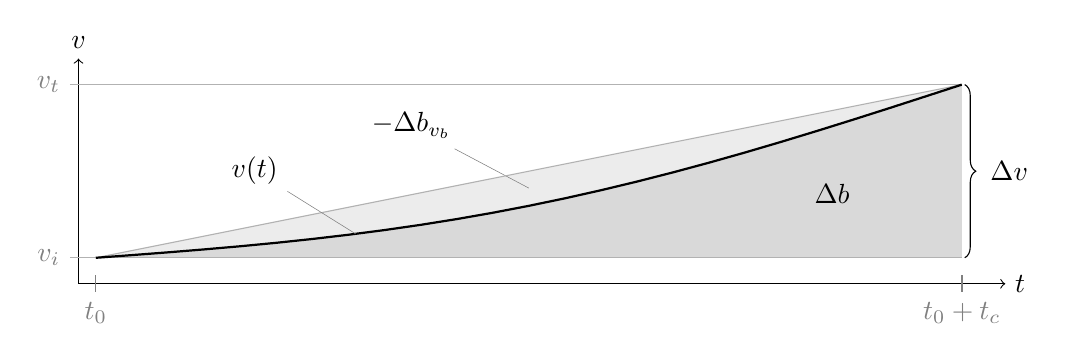
\begin{tikzpicture}[
	scale=11,
	pin distance=10mm,
	pin position=150]

\tikzstyle{subtle}=[thin,gray]
\tikzstyle{subtle line}=[thin,gray!60]

\def\XOffset{-0.02}
\def\YOffset{0.03}
\def\LinearCoef{0.2}
\def\NonlinearCoef{-0.04}
\pgfmathsetmacro{\InitialTempo}{\YOffset}
\pgfmathsetmacro{\TargetTempo}{\YOffset + \LinearCoef}
\pgfmathsetmacro{\PlotHeigth}{2 * \YOffset + \LinearCoef}
\pgfmathsetmacro{\CenterTempo}{\YOffset + 0.5 * \LinearCoef}

% Draw axes
\draw [<->] (\XOffset, \PlotHeigth) node (yaxis) [above] {$v$}
	|- (1.05,0) node (xaxis) [right] {$t$};

% ticks on time axis
\draw[subtle] (0,0.01) -- (0,-0.01) node [below] {$t_0$};
\draw[subtle] (1,0.01) -- (1,-0.01) node [below] {$t_0 + t_c$};

% non-linear position change
\path[fill=gray!15]
	(0, \InitialTempo)
	-- (1, \TargetTempo)
	-- (1, \InitialTempo)
	-- cycle;
\node at (0.5, 0.85 * \CenterTempo) [coordinate,
	pin=$-\Delta b_{v_b}$
	] {};

% Total position change
\path[fill=gray!30,domain=0:1]
(0, \InitialTempo) --
plot (\x,
{
	\YOffset +
	\LinearCoef * \x +
	\NonlinearCoef * sin(pi * \x r)
}) --
(1, \InitialTempo) --
cycle;
\node at (0.85, 0.8 * \CenterTempo) {$\Delta b$};

% line for linear tempo change
\draw[subtle line]
(0, \InitialTempo) --
(1, \TargetTempo);

% Initial tempo
\draw[subtle line]
(\XOffset - 0.01, \InitialTempo) node[left, subtle] {$v_i$} -|
(1, \InitialTempo);

% Target tempo
\draw[subtle line]
(\XOffset - 0.01, \TargetTempo) node[left, subtle] {$v_t$} -|
(1, \TargetTempo);

% Tempo change
\draw [decorate,decoration={brace,mirror,amplitude=4pt,raise=1pt},yshift=0pt]
	(1, \InitialTempo) -- (1, \TargetTempo)
	node [black,midway,xshift=0.6cm] {$\Delta v$};

% actual function
\pgfmathsetmacro{\FunctionLabelPos}{
	\YOffset +
	\LinearCoef * 0.3 +
	\NonlinearCoef * sin(pi * 0.3 r)}
\draw[thick,domain=0:1]
plot (\x,
{
	\YOffset +
	\LinearCoef * \x +
	\NonlinearCoef * sin(pi * \x r)
});
\node at (0.3, \FunctionLabelPos) [coordinate,
	pin=$v(t)$
	] {};

\end{tikzpicture}
\caption{
Tempo function $v(t)$,
showing the total tempo change $\Delta v$,
total position change $\Delta b$,
and position change caused by the non-linear
part of the tempo function, $\Delta b_{v_b}$.
Also visible are the initial and target tempi,
$v_i$ and $v_t$ respectively.
}
\label{fig:tempo_function}
\end{center}
\end{figure}

\subsubsection*{Correcting tempo differences}

To make a tempo change
over $t_c$ equal to $\Delta v$,
we define the tempo changing part of our tempo function
\begin{equation}
\label{eq:tempo_function_tempo_correction}
v_t(t) =
\begin{cases}
\frac{\Delta v}{t_c} \, t & \text{if } t < t_c \\
\Delta v & \text{otherwise}.
\end{cases}
\end{equation}
Since the tempo is changed gradually,
it will not immediately match the target tempo.
The difference to the target tempo causes
a cumulative difference in position,
which can be simply solved by integrating over time:
\begin{equation}
\label{eq:linear_tempo_change_pos_diff}
\int v_t - \Delta v \, \mathrm{d}t =
\Delta v \left( \frac{t^2}{2 \, t_c} - t \right) + C.
\end{equation}
The difference in position
caused by the difference between $v_t(t)$ and $\Delta v$
cumulates over the catchup time $t_c$,
causing a gross difference of
\begin{equation}
\Delta b_{v_t} =
\int_t^{t + t_c} v_t - \Delta v \, \mathrm{d}t =
-\frac{\Delta v \, t_c }{2}.
\end{equation}
This difference in position will need to be taken into account
when defining $v_b(t)$,
which should compensate for the position difference.

\subsubsection*{Correcting position differences}

To have an effect on position,
but zero effect on the final tempo,
we define the position changing part of our tempo function
\begin{equation}
v_b(t) =
\begin{cases}
a \sin \left( \frac{\pi t}{t_c} \right) & \text{if } t < t_c \\
0 & \text{otherwise},
\end{cases}
\end{equation}
where $a$ is the correction coefficient
contributing to the amount of change in position.
To solve $a$, we need to look at the
cumulative position difference caused by $v_b(t)$,
which can be solved from the integral
\begin{equation}
\int v_b \, \mathrm{d}t =
\frac{a t}{\pi} \left( 1 - \cos \left( \frac{\pi t}{t_c} \right) \right) + C.
\end{equation}
Similarly to $\Delta b_{v_t}$,
the gross difference in position caused by $v_b$ over $t_c$
\begin{equation}
\label{eq:non-linear_tempo_func_total}
\Delta b_{v_b} = \int_t^{t + t_c} v_b \, \mathrm{d}t =
\frac{2 \, a \, t_c}{\pi}.
\end{equation}
To completely correct the position after $t_c$,
$v_b$ will need to both compensate for
$\Delta b$ and counter the positional change caused by $v_t$,
giving the equation
\begin{equation}
\Delta b_{v_b} = - \left( \Delta b + \Delta b_{v_t} \right) .
\end{equation}
Thus, applying equation \ref{eq:non-linear_tempo_func_total},
we can solve $a$ as
\begin{equation}
\label{eq:non_linear_coef}
a = - \frac{\pi \left( \Delta b + \Delta b_{v_t} \right)}{2 t_c}.
\end{equation}

\subsection{Offset Compensation}

Given the previous beat offset $\Delta b'$ (at time $t'$),
and current $v_t$ and $v_b$,
the current offset can be estimated as
\begin{equation}
\label{eq:tempo_function_offset_function}
\Delta b(t) = \Delta b' - \int_{t'}^t v_t + v_b \, \mathrm{d}t.
\end{equation}
To get the best beat classifications,
$ \mathcal{C} $ is used with the relative beat position
\begin{equation}
b' = \mathcal{M} [ t ] - p_B - \Delta b(t),
\end{equation}
where $t$ is the time of the beat,
and $p_B$ the beginning of the current bar.
The offset approaches zero as $t$ approaches $t' + t_c$.

\subsection{Tempo Changes}

\fixme{Revise once the method use is final!}

Tempo changes in the score are taken into account
by changing the tempo function accordingly.
When the tempo changes by a factor $a$,
new values for $\Delta v$ and $\Delta b$ are calculated,
and the tempo function is reset.
The new change in tempo
\begin{equation}
\Delta v = a \left( v_i' + \Delta v' \right) - v'(t),
\end{equation}
where $v_i'$ is the previous initial tempo,
$\Delta v'$ the previous tempo change,
and $v'(t)$ the current tempo.
The new offset
\begin{equation}
\Delta b = \Delta b'(t),
\end{equation}
where $\Delta b'(t)$ is the previous offset function
as defined in equation \ref{eq:tempo_function_offset_function},
is expressed in beats,
and is thus not affected by the tempo change.

When changing a tempo function that has not yet
finished applying its changes,
the most intuitive course of action would be to set
\begin{equation}
\label{eq:tempo_change_bad_tc}
t_c = t_c' - t,
\end{equation}
where $t_c'$ is the previous value of $t_c$,
and $t$ the time since the function was last reset.
However, since $\Delta v$ will be finite in most cases,
we can see that the coefficient $\frac{\Delta v}{t_c}$
in equation \ref{eq:tempo_function_tempo_correction}
will approach infinity,
as $t$ approaches $t_c'$:
\begin{equation}
\lim_{t \to t_c'} \frac{\Delta v}{t_c' - t} = \pm \infty,
\, \Delta v \neq 0.
\end{equation}
Thus it is not feasible to use equation \ref{eq:tempo_change_bad_tc},
but we instead define $t_c = t_c'$.

\subsection{Relaxed Tempo Following}

Since the tempo adjustment function defined in
\ref{sec:tempo_function} is non-linear,
selecting the catchup time $t_c$ properly is critical.
To have a consistent state for each beat estimation,
the adjustment should be fully completed
or very near completion
at the time the next beat occurs.
A very short time, however,
would cause very abrupt changes in tempo.
Thus $t_c$ is selected as the time between
the current and previous beat,
which should predict the time to the next
beat fairly well.

The tempo adjustment method described above is very strict,
as it attempts to do a full tempo and position correction
between each beat.
In a real life situation
the timing of the detected beats will often have some
fluctuation over time,
causing large beat offsets.
When such an offset is present,
the non-linear part of the tempo function,
trying to correct the offset,
will cause a large temporary change in tempo.

It is not viable to filter the beat offset values,
as is done with the instantaneous tempi,
for the offset is directly affected by
the tempo adjustment function.
Doing so would cause feedback in the system,
with hard to predict results.
Instead, only part of the beat offset is compensated for.
This adjustment does not apply to
the offset caused by the tempo change
(equation \ref{eq:linear_tempo_change_pos_diff}),
but only the offset of the latest beat.
To relax the tempo following,
only a fraction of the beat offset $\Delta b$ is corrected,
modifying the coefficient for the non-linear 
part of the tempo function, defined in equation
\ref{eq:non_linear_coef}.

\section{Start Tempo Estimation}
\label{sec:meth:start_tempo_estimation}

The start tempo is estimated based on
the duration of the start gesture.
As there are several beat patterns for a given time signature,
the length of the start gesture may also differ.
The duration from bottom to top position is
assumed to be half the length of
the first \textit{conducted} beat.
The starting tempo is thus
\begin{equation}
v_s = \frac{\Delta t_{b_{1,2}}}{2} (t_t - t_b),
\end{equation}
where $\Delta t_{b1,2}$ is the
time between the first and second conducted beat,
$t_t$ the time at the top of the gesture,
and $t_b$ the time at the bottom of the gesture.
From the different values of $v_s$ derived from the
different conducting patterns,
the one closest to the transcribed tempo is selected
as the final start tempo.


%%%%%%%%%%%%%%%%%%%%%%%%%%%%%%%%%%%%%%%%%%%%%%%%%%%%%
\chapter{Sound Synthesis}
\label{chapter:sound_synthesis}

Since the objective of the system is to emulate an orchestra,
also the sound synthesis system should be able to
provide realistic synthesis of an entire orchestra.
It should be able to reproduce a musical composition
at varying tempi and articulations.
To support these requirements,
the most straightforward approach is to use
a score defined as a set of score events
(notes, tempo events, etc.),
which function as the input to a synthesis engine,
which produces the final output sound in real time.
The score event format needs to be in,
or convertible to a format that is understood by the synthesis engine.
This means the score format is most tightly
coupled to the synthesis engine,
while the coupling to the rest of the system is rather loose.
The synthesis engine and score format selected for the system
are presented in this chapter.

\section{Vienna Symphonic Library}

There are several commercial orchestral synthesizers available,
the majority of which use some form of sampling or concatenative synthesis.
Based on the feature set provided and
subjective evaluation of sound quality,
Vienna Symphonic Library (VSL) \cite{vsl} was chosen for the task.
VSL uses a form of concatenative synthesis,
using a vast library of samples played at
various velocities and articulations \cite{schwartz2006}.

Each instrument in VSL contains a set of \textit{patches},
which represent a certain articulation and/or playing style.
Each patch is capable of synthesizing
the whole scale of the given instrument at several velocities.
Some patches (such as \textit{staccato} articulations)
have a limited note length,
while others allow stretching out the note infinitely.
Switching between patches can be accomplished with \textit{keyswitch} events.

VSL also contains a \textit{Multi Impulse Response Mixing and Reverberation}
engine (MIR).
MIR allows simulating an acoustic environment with
the possibility of placing virtual instruments and microphones
rather freely in a room.
MIR includes impulse response data for the Vienna Konzerthaus,
and allows placing the virtual microphones at the conductor's podium.

\subsection{Virtual Studio Technology}
\label{sec:vst}

Virtual Studio Technology (VST) \cite{vst} is
a virtual instrument and effect plugin architecture created by Steinberg GmbH.
It is one of the plugin formats that VSL is available in.
While the plugin API should be considered an implementation detail,
it can not be completely ignored in the design phase,
because of the vast effect design choices can have on implementation complexity.
VST will be referred to in later parts of this document,
and is thus introduced here.

\section{Score Event Format}

In order to play a score,
the score events need to be provided to the system in some format.
The objective was to be able to use existing material as much as possible,
with minimal effort.
The format used in the system combines
a MIDI score, discussed in section \ref{sec:midi} and
a terse domain specific language (DSL) based score description format,
discussed in section \ref{sec:score_description_file}.

\subsection{The Musical Instrument Digital Interface}
\label{sec:midi}

Regardless of its limitations and age,
the Musical Instrument Digital Interface (MIDI)
is still one of the most used standards
for the digital representation of musical events.
MIDI is also the built-in way to communicate musical events
in the Virtual Studio Technology (VST) plugin format.
Thus using MIDI as the score format is a natural choice.

A MIDI score contains note, time signature and tempo information.
It may also contain \textit{program change} events,
as specified in the General Midi specification \cite{GeneralMidi},
to indicate the instrument to be used for each track.
However, practical experience with MIDI files showed,
that using program changes to deduce the instrument to use,
was not sufficient.
Often scores would use the
\textit{String ensemble} patch for all strings,
even though the string instruments were separated to individual tracks.
In cases like this it is necessary to be able to manually
define the instrument to be used with each track.
See section \ref{sec:score_description_file}.

\section{Patch Switching}
\label{sec:patch_switching}

In order to control the switching of patches,
the synthesis system must have some knowledge of
the available instruments and their patches.
The parameters used for describing the patches are:
\begin{description}
\item[Length] The maximum note length allowed by the patch.
\item[Attack] The sharpness of the attack portion of the notes.
\item[Weight] The \textit{musical weight} of the note, i.e. an accented note would have a large weight.
\end{description}
By using this information,
together with the current motion capture and score state,
the system is capable of selecting
the most appropriate patch for each note.

\fixme{Write more on patch selection (e.g. distance function)}

%%%%%%%%%%%%%%%%%%%%%%%%%%%%%%%%%%%%%%%%%%%%%%%%%%%%%
\chapter{Visualization}
\label{chapter:visualization}

During the development of the conductor follower,
a good mechanism for observing the state of the system
in real time was lacking,
which eventually lead to developing a real time visualization.
While the visualization provided its greatest benefits
during the development of the system,
it can also provide valuable feedback to users of the system.
This chapter discusses the functionality
and motivation behind each visualization feature separately.

\section{Movement Tracing}

When conducting a pattern,
it is very difficult for the conductor himself to
perceive the actual shape of the hand movement.
These days it is common practice to 
videotape the rehearsals of conducting students \cite{?}
for the students to better see how they perform.
However, this method does not provide an
immediate form of feedback during the rehearsal.

By visualizing both the current position of the hand,
and a trace of the movement history,
immediate visual feedback can be provided.
An intuitive way of presenting the movement history
is to draw a colored line segment between each sampled position,
with the opacity of the segment decreasing the older the samples are.

\section{Spatial Beat Visualization}

The visualization can show the spatial position
of the detected beats,
which occur along the traced hand trajectory.
Due to the nature of the beat detection algorithm --
which does not represent an absolute truth about
how beats should be detected --
the usefulness of this visualization for
pedagogical purposes is questionable.
However, the visualization was a good aid
during the development of the system,
and could be a good aid if the system is to be developed further.

\section{Beat Offset Visualization}

To indicate the positions of the detected beats
relative to their classifications,
a circular visualization is used.
The progress of the current bar
is visualized with a segment of a circle,
alternately growing to a full circle,
and shrinking to zero length,
as the bar progress to their ends.
The detected beats are visualized outside this circle,
as a segment from the detected position
to the position of the respective classification.
Beats that happened early are visualized in green,
and beats that happened late in red.
Similarly to the movement tracing,
the opacity of the old beats decreases
and they eventually disappear as time progresses.

\section{Depth Sensor Output}

In addition to visualizations which describe
the state of the conductor follower,
the raw output of the depth sensor can be displayed
as a grayscale video.
This is mainly useful for solving possible issues
related to the way the depth sensor works:
In some situations infra red sources,
such as the sun,
or certain hand positions
can cause problems with the hand tracking algorithm.
The depth sensor output can in some situations help
in identifying and possibly correcting these problems.


%%%%%%%%%%%%%%%%%%%%%%%%%%%%%%%%%%%%%%%%%%%%%%%%%%%%%
\chapter{Implementation Details}
\label{chapter:implementation_details}

Since the synthesis environment is a
Virtual Studio Technology (VST) plugin,
implementing the conductor follower as a VST plugin was a logical choice.
The input for the plugin is read from a MIDI file
and the output is MIDI events via the VST interface.
These implementation details are, however, hidden behind
carefully designed interfaces,
separating the core functionality from the input/output functionality.

One of the most important considerations of the implementation
is its real-time (RT) constraints.
A RT system is defined as a system where calculations
need to be completed before a given deadline,
and can be classified into three categories:
\begin{description}
\item[Hard]
Missing a deadline is a total system failure.
\item[Firm]
The usefulness of a result is zero after its deadline.
\item[Soft]
The usefulness of a result degrades after its deadline.
\end{description}
An audio plugin has firm real-time constraints,
since the result for each block of audio needs to be delivered in time.
Missing a deadline means that block will not be played back,
causing a glitch in the sound output.

It is important to understand the difference between
deadline based real time constraints
and throughoutput based constraints.
Throughoutput based real time constraints have
more to do with with the algorithmic complexity
of the methods used,
while deadline based constraints
require special programming techniques on the implementation level.
All further references to RT constraints in this thesis
refer to the deadline based definition.

In addition to having RT constraints,
the 30Hz frame rate of the motion capture system
makes it a multirate, multithreaded application.
Working in such an environment requires using
lock-free programming techniques,
such as atomic variables and lock-free ringbuffers.
The multirate nature also requires having robust timestamping and synchronization mechanisms.

\fixme{chapter overview}

\section{Supporting Libraries}
\label{sec:supporting_libraries}

The implementation makes heavy use of several of the Boost C++ libraries \cite{boost}.
The most noteworthy ones are described in the following list.
Libraries included in the C++11 standard \cite{cpp11}
are denoted with $^*$,
while libraries not yet in the official boost distribution
are marked with $^\dagger$.
\begin{description}[leftmargin=14ex]
\item[Chrono$^*$] Time library for timestamping and jitter correction.
%\item[Geometry] Is this really used much anywhere?
\item[Lockfree$^\dagger$] Various lock-free constructs.
\item[Spirit] A parsing library, used for configuration file parsing.
\item[Thread$^*$] Threading utilities.
\item[uBLAS] Linear algebra, used for polynomial fitting.
\item[Units] Compile-time dimensional analysis.
\end{description}

The OpenNI Framework \cite{openni} is an open source cross-platform
framework for Natural Interaction (NI) devices.
PrimeSense Ltd \cite{primesense} provides a proprietary
middleware package called NITE,
which works with the OpenNI API,
providing higher level functionality such as skeletal and hand tracking.
NITE is used via the OpenNI APIs for hand tracking.

Juce \cite{juce} is an open source,
multimedia oriented cross-platform C++ library.
It was used for its
VST plugin wrapper, MIDI file I/O,
and user interface (UI) functionality.

\section{Architectural overview}

The implementation is divided into
six well defined and loosely coupled modules:
\begin{itemize}
\item Common utilities
\item Data file parsers
\item Motion capture
\item Expression to synthesis parameter mapper
\item Score Follower (the core functionality)
\item The VST plugin
\end{itemize}

The common utilities module contains components
that are not specific to conductor following.
These include utilities for
lock-free programming,
mathematical operations and algorithms,
time and geometry handling,
logging, and debugging.

The data file parser module
contains all the parser definitions
and supporting data structures
for all the input files used by the system.
Its main purpose is to hide the implementation
of parsing behind a concise API.

The motion capture module provides a simple
event-based API for motion related data.
It includes the logic for extracting relevant events from motion data.
It also contains all the code that uses the OpenNI APIs,
so that the rest of the system has no dependencies on OpenNI.

The expression to synthesis parameter mapper
maps expression parameters to synthesis parameters.
\fixme{Write more}

The score follower module provides most of the core functionality,
not including motion capture.
This includes
beat classification, tempo and score following, jitter correction,
and instrument patch switching among other things.
It also provides abstract interfaces for 
hiding the implementation details of the score format.

The VST plugin modules main purpose is to
separate as much plugin implementation detail from the rest of the system.
It implements the VST interface and provides the plugin UI,
both using Juce.
It also implements the score related interfaces,
defined in the score follower module,
using Juce MIDI functionality.

In addition to these six modules,
the project contains four unit test modules.
These modules are not significant regarding the functionality,
but merely had a supporting role during system development.

\subsection{Thread model}

The VST architecture implies using at least two threads:
one for audio and/or MIDI processing,
and another for the UI.
In addition to these two threads,
motion capture needs it's own thread,
and one additional thread is needed for some
lockfree programming techniques.
To summarize, the threads are:
\begin{enumerate}

\item VST MIDI (audio)
\begin{itemize}
\item Provided by plugin host.
\item Produces the MIDI events.
\item Has firm RT requirements.
\item Low latency required.
\end{itemize}

\item VST UI
\begin{itemize}
\item Provided by plugin host.
\item Renders the plugin UI.
\end{itemize}

\item Motion Capture
\begin{itemize}
\item Runs the motion capture device.
\item Has firm RT requirements.
\item Higher latencies allowed compared to the MIDI thread (30 Hz).
\end{itemize}

\item Butler
\begin{itemize}
\item Runs asynchronous tasks for the RT threads.
\end{itemize}

\end{enumerate}

\subsection{Essential Common Utilities}

A number of utilities are widely used across the application,
and reserve a mention.
These are mostly related to lockfree programming techniques.

\subsubsection*{Event Buffer}

The event buffer is probably the most used utility in the implementation.
It is a container for storing timestamp-event-pairs.
It allows specifying the internal storage depending on the use case.
For data which is collected when loading the score,
a dynamically resizeable container (such as std::vector) can be used,
while buffers used during playback mostly use a statically sized ringbuffer
to guarantee allocation free operation.
Utilities for accessing timestamp-based ranges,
with all valid combinations of
bounded, left-bounded, left-open and left-closed are available.

\subsubsection*{The Butler Thread}

The butler thread is used for asynchronously running
tasks that can not be run in an RT-thread.
The butler thread is configured with a maximum execution interval,
and will check for new tasks and execute them repeatedly,
until terminated.
The thread will block as necessary to not exceed the
maximum execution interval.

\subsubsection*{Lockfree Ringbuffer}

The lockfree ringbuffer provided by the Boost.Lockfree library \cite{required?}
is used for most of the lockfree inter-thread communication.
This includes passing events from the motion capture thread
to the MIDI thread, and logging from RT threads using the Butler thread.
It is an essential utility for lockfree multi-threaded programming.

\subsubsection*{Chen \& Burns Buffer}

While the lockfree ringbuffer is a good solution
for event-like data,
better mechanisms exist for sharing a a single
instance of data, e.g. a state. 
For this use, a fully asynchronous reader-writer mechanism
as described by Chen and Burns \cite{Chen97} was implemented.
The mechanism allows lockfree access for
a single writer and a fixed number of readers.
It uses a number of copies of the data,
and a set of atomic variables to track
the reading and writing states.


\section{Time Handling}
\label{sec:time_handling}

Handling time in a multirate, multi-threaded system,
is not a trivial task.
The motion capture thread will be in
a blocking state most of the time,
waking up at a 30Hz frequency to process data
provided by the motion capture system.
The plugin, however, needs to provide MIDI data
based on the host's audio settings,
a typical configuration running the
plugin at around 100 Hz (an audio block length of 10ms).
Additionally, the thread in which the plugin runs
is controlled by the host,
and the code has to be completely lock-free.

Considering the implications of needing to run lock-free code on
a modern multi-core system, running a general purpose
operating system (OS),
no assumptions about causality or parallelism between
motion capture and plugin code execution can be made --
scheduling latencies and parallel execution forces the use
of a reliable timestamping mechanism for synchronization between
the audio and motion capture threads.
The Boost Chrono library provides a steady clock,
which measures time since the latest system boot-up.
Acquiring the current timestamp was verified to be lock-free
at least on Windows and OS X as of Boost version 1.49.0.
These timestamps are used for measuring the interval between
events happening in the motion capture and plugin threads.
Timestamping events in the motion capture thread is straightforward,
each event simply being timestamped with
the current timestamp returned by the system.
The plugin thread will, however,
require jitter correction to prevent timing problems.

\subsection{Jitter Correction}

The plugin thread needs to know not only
the timestamp corresponding to the beginning of the current audio block,
but also an estimate for the end of the block.
Let the audio block be defined by its beginning and end:
\[
\boldsymbol{\tau} \definedas [\tau_b, \tau_e[.
\]
Using the information provided to the plugin,
the theoretical block length
\begin{equation}
\label{eq:theoretical_block_len}
\Delta \tau' = \frac{n_b}{f_s},
\end{equation}
where $n_b$ is the block size in samples and $f_s$ the samplerate.
This length is then used for estimating the end of each block
\begin{equation}
\tau_e = t_c + \Delta \tau',
\end{equation}
where $t_c$ is the current timestamp at the beginning of the block.
Due to scheduling latencies,
the value of $t_c$ might differ from the
previous block end estimate $\tau_{e_{\mathrm{prev}}}$.
In order to prevent gaps and overlaps between the
time estimates of consecutive audio blocks,
the beginning of each block is taken from the end of the previous block
\begin{equation}
\tau_b = \tau_{e_{\mathrm{prev}}}.
\end{equation}
The VST specification requires
each MIDI event to have its position defined
as a sample offset from the beginning of the current block.
As the actual block length
\begin{equation}
\Delta \tau = \tau_e - \tau_b
\end{equation}
will differ from the theoretical block length
$\Delta \tau'$ most of the time,
this difference will need to be taken into consideration
when calculating the event sample offset
\begin{equation}
\Delta n_e = \frac{\Delta \tau'}{\Delta \tau} (t_e - \tau_b) f_s,
\end{equation}
where $t_e$ is the event time. By using equation \ref{eq:theoretical_block_len},
this can be simplified to
\begin{equation}
\Delta n_e = n_b \frac{t_e - \tau_b}{\Delta \tau}.
\end{equation}

\subsection{Dimensional Analysis}

Because of the various time bases and units used
(see section \ref{sec:meth:read_and_score_time}),
using compile time dimensional analysis using Boost.Units \cite{needed?}
eased the development process.
Boost.Units uses zero runtime overhead C++ template metaprogramming \cite{abrahams?}
techniques to check during compile time,
that all calculations have the proper dimensions.
This does not guarantee dimensionally proper calculations all the time
(e.g. dimensionless units may cause errors),
but does catch many errors made during development.
For handling time,
a custom unit system was declared.
This system contains base dimensions for
beats, bars, samples and physical time,
and derived dimensions for
bar durations, tempi, sample rates, and speed changes.
The unit system is described in detail in Table \ref{tab:score_units}.
The difference between physical time and score time (both in seconds),
comes inherently from the libraries used:
Boost.Units for score time and Boost.Chrono for physical time.
This implies that an explicit conversion function is always
needed to convert between these two dimensions.

\begin{table}
\begin{center}
\begin{tabular}{ | l  l  p{5.5cm} |}
\hline
Dimension & Base Unit & Notes \\ \hline
beats & beat & Base for musical time \\
bars & bar & See bar duration. \\
samples & sample & See sample rate\\
time & second & Base for physical time \\
bar duration & beats per bar & Derived dimension. \\
tempo & beats per second & Derived dimension. \\
sample rate & samples per second & Derived dimension. \\
speed change & fractions per second & Fraction here is a dimensionless unit. A derived dimension. \\
\hline
\end{tabular}
\caption{Overview of custom unit system for time.}
\label{tab:score_units}
\end{center}
\end{table}

\section{Motion Capture}

\subsection{The Polynomial Regression Filter}

The polynomial regression filter is used for three purposes in the system:
smoothing, differentiation and interpolation.
The polynomial fitting part for the filter is implemented using
matrix operations and the uBLAS library.
Estimating the polynomial coefficients is done by the equation
\begin{equation}
\label{eq:sg_coefs}
\widehat{\mathbf{a}} = \left( \mathbf{X}^T \mathbf{X} \right)^{-1} \mathbf{X}^T \mathbf{y},
\end{equation}
where $\widehat{\mathbf{a}}$ are the estimated coefficients,
$\mathbf{y}$ the observations,
and $\mathbf{X}$ the design matrix
\begin{equation}
\label{eq:sg_design_matrix}
\mathbf{X} = \left[
\begin{array}{ccccc}
1 & x_1 & x_1^2 & \ldots & x_1^m \\
1 & x_2 & x_2^2 & \ldots & x_2^m \\
1 & x_3 & x_3^2 & \ldots & x_3^m \\
\vdots & \vdots & \vdots & & \vdots \\
1 & x_n & x_n^2 & \ldots & x_n^m \\
\end{array}
\right] ,
\end{equation}
where $x_1 \ldots x_n$ are the observation times,
and $m$ the order of the resulting polynomial.
It is required that $n > m$.
Smoothing and differentiation is implemented by
selecting an odd value for $n$
and evaluation the polynomial at the center value
$x_{\lfloor \frac{n}{2} \rfloor}$.
An optimization that is easy to implement for equally sampled data,
is to pre-calculate $\left( \mathbf{X}^T \mathbf{X} \right)^{-1} \mathbf{X}^T$,
with $x_{\lfloor \frac{n}{2} \rfloor} = 0$.
The value and derivatives at the center point
can thus be calculated from the polynomial
\begin{equation}
\widehat{y}(x) =
\widehat{\mathbf{a}}_m \, x^m +
\widehat{\mathbf{a}}_{m-1} \, x^{m-1} +
\ldots +
\widehat{\mathbf{a}}_{2} \, x +
\widehat{\mathbf{a}}_{1}.
\end{equation}
The simplified equations being
\begin{equation}
\widehat{y}(0) = \widehat{\mathbf{a}}_{1}
\end{equation}
for the value, and
\begin{equation}
\widehat{y}^{(n)}(0) = n! \: \widehat{\mathbf{a}}_{n + 1}
\end{equation}
for the \nth derivative.

To make $\mathbf{X}^T \mathbf{X}$ invertible,
it is also necessary to reverse the values $x_1 \ldots x_n$
used in equation \ref{eq:sg_design_matrix}.
This change requires a correction to equation \ref{eq:sg_coefs},
which is reversing the observation values $\mathbf{y}$.

\section{Data File Formats}

For additional data needed by the system,
a number of JSON-like \cite{JSON} DSLs were developed.
The syntax in all of them is similar,
only the contained data varying between different formats.
The formats will be described here briefly.

\subsection{Score Description Files}
\label{sec:score_description_file}

Because the data present in a MIDI score was
not sufficient alone, a format
for describing additional data related to the score was developed.
A score definition file includes the following information:
\begin{description}[leftmargin=24ex]
\item[Name] A human readable name for the score.
\item[MIDI file] The path of the related midi file.
\item[Instrument file] The path of the related instrument definition file.
\item[Beat pattern file] The path of the related beat pattern file.
\item[Track information] A list of track to instrument mappings.
\item[Score events] A list of score event.
\end{description}
An example of a score description file can be found from Appendix \ref{appendix:dsl_samples}.
For more information on instrument definitions,
see section \ref{sec:instrument_definition_format},
and for beat patterns section \ref{sec:instrument_definition_format}.
The different types of score events are described in detail below.

\subsubsection*{Tempo Sensitivity Events}

A tempo sensitivity event contains the following information:
\begin{description}[leftmargin=16ex]
\item[Position] The score position to which this sensitivity change applies.
\item[Sensitivity] A sensitivity value in the range $0 \ldots 1$.
\end{description}
The event will cause the catchup time $t_c$,
as described in section \ref{sec:tempo_function},
to be adjusted to provide a different level of sensitivity in tempo following.
A low sensitivity will lead to a long $t_c$,
whereas a high sensitivity translates to a short $t_c$.

\fixme{If no more events are implemented, change the formatting}

\subsection{Instrument Definition Files}
\label{sec:instrument_definition_format}

The purpose of instrument definition files,
is to provide the necessary data for
mapping expressive parameters to different
instrument patches.
The file is a list of instrument definitions,
which include patch definitions.
A patch definition includes the following information:
\begin{description}[leftmargin=24ex]
\item[Name] A human readable name for the patch.
\item[Keyswitch] The keyswitch for selecting this patch.
\item[Length] Length of patch, as described in section \ref{sec:patch_switching}.
This is a relative value in the range \ocinterval{0, 1}.
\item[Attack] Attack of patch, as described in section \ref{sec:patch_switching}.
\item[Weight] Weight of patch, as described in section \ref{sec:patch_switching}.
\end{description}
Each patch is unique to an instrument,
the instrument definition including the following information:
\begin{description}[leftmargin=24ex]
\item[Name] A human readable name for the instrument.
\item[Shortest note] The length for the relative note length of 0.
\item[Longest note] The length for the relative note length of 1.
\item[Patches] List of patches.
\end{description}
An example of an instrument definition file can be found from Appendix
\ref{appendix:dsl_samples}.

\subsection{Beat Pattern Definition Files}
\label{sec:beat_pattern_definition_format}

The beat pattern definition files include the
information for all the conducting beat patterns
that the system recognizes.
Each beat pattern includes the following information:
\begin{description}[leftmargin=24ex]
\item[Meter] The time signature to which this pattern applies.
\item[Beats] A list of beat times as an offset into the bar in quarter notes.
\end{description}
An example of a beat pattern definition file can be found from Appendix
\ref{appendix:dsl_samples}.

%%%%%%%%%%%%%%%%%%%%%%%%%%%%%%%%%%%%%%%%%%%%%%%%%%%%%
\chapter{Discussion and Conclusions}
\label{chapter:discussion}

\fixme{Summarize}

\section{Evaluation of Results}

\fixme{Write}

\section{Further work}

\fixme{Write}

\subsection{Motion Tracking}

\fixme{Write}

\subsection{Score Analysis}

\fixme{Write}

\section{Conclusions}

\fixme{Write}